\documentclass{beamer}

\usepackage[noend]{algpseudocode}

\usepackage{algorithmicx,algorithm}
\usepackage{pgfpages}
%\setbeameroption{show notes}
%\setbeameroption{show notes on second screen=right}
\mode<presentation> {
  \usetheme{Darmstadt}
  %\setbeamercovered{transparent}

 %\setbeamertemplate{background canvas}[vertical shading][bottom=red!10,top=blue!10]

 \setbeamertemplate{blocks}[rounded][shadow=true]
 %\usetheme{Warsaw}

\expandafter\def\expandafter\insertshorttitle\expandafter{%
	\insertshorttitle\hfill%
	\insertframenumber\,/\,\inserttotalframenumber}
 
 \setbeamercovered{transparent}
 \setbeamertemplate{footline}[frame number]
 \usefonttheme[onlysmall]{structurebold}
 %\useoutertheme{infolines}
 \usefonttheme[onlymath]{serif}
}


\usepackage{array}
\usepackage{amsfonts}
\usepackage{indentfirst}
\usepackage{color}
\usepackage[french]{babel}
\usepackage{graphicx}
\usepackage[latin1]{inputenc}
\usepackage{times}
\usepackage[T1]{fontenc}
\usepackage{tikz}
\usepackage{algorithmic}


\setbeamertemplate{footline}[frame number]


%%%%%%%%%%%%%%%%%%%%%%%%%%%
\title[SSIR reporting] 
{A convex formulation for high-dimensional sparse sliced inverse regression}


\author{Xiaolong Luo ,Ruoru Yan }

\institute[]
{
  
  School of management
  \and
 
  University of Science and Technology of China
 
}

\date 
{}



\begin{document}


\begin{frame}
  \titlepage
\end{frame}

\begin{frame}{Reporting Content}
  \tableofcontents
\end{frame}

\section{Abstract}

\subsection{Research context}
\begin{frame}{Object}
 \setlength{\parindent}{2em}  Sufficient dimension reduction by replacing covariates with \textcolor{blue}{a minimal set of their linear combinations} without loss of information 
  
  
 \setlength{\parindent}{2em} Assuming that the number (d) of stochastic covariate x exceeds the sample size n,we consider the following question:
 
 \begin{equation}
    y \perp x \mid\left(\beta_{1}^{\mathrm{T}} x, \ldots, \beta_{K}^{\mathrm{T}} x\right)
\end{equation}
  
  
  it equals to :
  \begin{equation}
     y=f\left(\beta_{1}^{\mathrm{T}} x, \ldots, \beta_{K}^{\mathrm{T}} x, \epsilon\right)
\end{equation}
\end{frame}

\begin{frame}{Object}
  From equation(2):
$$
    y=f\left(\beta_{1}^{\mathrm{T}} x, \ldots, \beta_{K}^{\mathrm{T}} x, \epsilon\right)
$$
\\
  \setlength{\parindent}{1em}y can be explained by a set of K linear combinations of x,and we henceforth refer to $\beta_{1}$,$\ldots$,$\beta_{K}$ as \textcolor{blue}{the sufficient dimension reduction directions} and define the intersection of the subspace spanned by them as \textcolor{blue}{the central subspace} $ V _{y|x} $    
\end{frame}

\subsection{Main Theory}
\begin{frame}{Three problem development}

  \textcolor{blue}{Linearity condition:} $ \forall a \in R^d $,
\begin{equation}
    E\left(a^{\mathrm{T}} x \mid \beta_{1}^{\mathrm{T}} x, \ldots, \beta_{K}^{\mathrm{T}} x\right)=b_{0}+b_{1} \beta_{1}^{\mathrm{T}} x+\cdots+b_{K} \beta_{K}^{\mathrm{T}} x
\end{equation}


With this condition,we have: 
\begin{equation}
    {\Sigma}_{E\left( x\mid y\right)} \beta_{k} = \lambda_{k}\Sigma_{x}\beta_{k}
\end{equation}

\\ \textcolor{red}{Problem 1:} a non-convex optimization problem:

\begin{equation}
   \underset{V \in \mathbb{R}^{d \times K}}{\operatorname{minimize}}-\operatorname{tr}\left\{V^{\mathrm{T}} \hat{\Sigma}_{E(x \mid y)} V\right\} \text { subject to } V^{\mathrm{T}} \hat{\Sigma}_{x} V=I_{K}
\end{equation}

\setlength{\parindent}{2em}With V represent a basis for $V_{y\mid x}$,we try to get a estimator of V by solving the following problem 1
\end{frame}

\begin{frame}{Three problem development}
\begin{itemize}
  \item {\color{red}{Problem 2:}} a convex relaxation problem:  $ \Pi = V V^\mathrm{T} $
\end{itemize}
  

\begin{equation}
 \underset{\Pi \in \mathcal{M}}{\operatorname{minimize}}-\operatorname{tr}\left\{\hat{\Sigma}_{E(x \mid y)} \Pi\right\}\\
 \quad\text { subject to }\left\|\hat{\Sigma}_{x}^{1 / 2} \Pi \Sigma_{x}^{1 / 2}\right\|_{*} \leqslant K,\left\|\hat{\Sigma}_{x}^{1 / 2} \Pi \hat{\Sigma}_{x}^{1 / 2}\right\|_{\mathrm{sp}} \leqslant 1  \quad   
\end{equation}


\begin{itemize}
    \item {\color{red}{Problem 3:}} adding the sparsity controlling parameter $ \rho $
\end{itemize}

\begin{equation}
 \underset{\Pi \in \mathcal{M}}{\operatorname{minimize}}-\operatorname{tr}\left\{\hat{\Sigma}_{E(x \mid y)} \Pi\right\}+\rho\|\Pi\|_{1} \\
 \quad\text { subject to }\left\|\hat{\Sigma}_{x}^{1 / 2} \Pi \hat{\Sigma}_{x}^{1 / 2}\right\|_{*} \leqslant K,\left\|\hat{\Sigma}_{x}^{1 / 2} \Pi \hat{\Sigma}_{x}^{1 / 2}\right\|_{\mathrm{sp}} \leqslant 1   \quad   
\end{equation}

\end{frame}



\section{Implementation}
\subsection{Approach}

\begin{frame}{Estimator for conditional covariance}
   \begin{itemize}
       \item We use $\operatorname{cov}\{E(x \mid y)\}=\operatorname{cov}(x)-E\{\operatorname{cov}(x \mid y)\}$ for estimation
       \item Let T = $E\{\operatorname{cov}(x \mid y)\}$ ,then, \color{red}{$\hat{\Sigma}_{E(x \mid y)}=\hat{\Sigma}_{x}-\hat{T}$}.
       \color{black}{We estimate T using following method:}
   \end{itemize}
    \begin{equation}
        \tilde{T}=\frac{1}{H} \sum_{h=1}^{H}\left\{\frac{1}{n_{h}} \sum_{i \in S_{h}}\left(x_{i}-\bar{x}_{S_{h}}\right)\left(x_{i}-\bar{x}_{S_{h}}\right)^{\mathrm{T}}\right\}
    \end{equation}
    \begin{itemize}
        \item We partition the n observations into H slices and compute the weighted average of the sample covariance matrices within each slice.
    \end{itemize}
\end{frame}

\begin{frame}{Estimator for conditional covariance}
  \textcolor{blue}{Code:}\\
  \centering 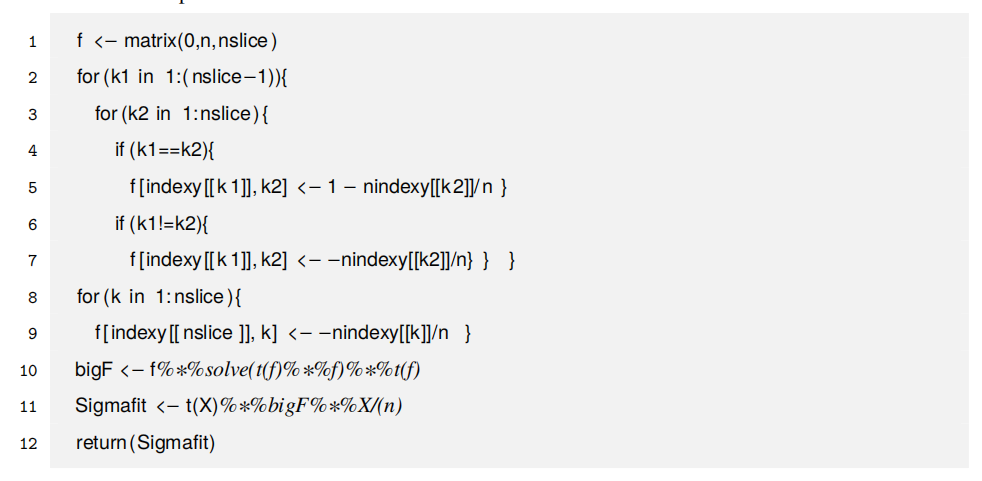
\includegraphics[scale=0.3]{code1}
\end{frame}

\begin{frame}{Algorithm for L-ADMM}
  \begin{algorithm}[H]
\caption{Linearized alternating direction of method of multipliers algorithmn}

\KwIn{ $\hat{\Sigma}_{x}, \hat{\Sigma}_{E(x \mid y)},$  tuning parameter $\rho,$ rank constraint $K,$ the L-ADMM parameters $v,$ tolerance level $\epsilon>0,$ and $\tau=4 v \lambda_{\max }^{2}\left(\hat{\Sigma}_{x}\right),$ }
%\KwOut{output result}%输出

\textbf{Initializations:  }primal variables $\Pi^{(0)}=I_{d}, H^{(0)}=I_{d}$, and dual variable $\Gamma^{(0)}=0$.\;
\end{algorithm}
\end{frame}

\begin{frame}{Algorithm for L-ADMM}
\begin{algorithm}[H]
\While{  $\left\|\Pi^{(t)}-\Pi^{(t-1)}\right\|_{\mathrm{F}} \geqslant \epsilon$. } \\
{\ a. \begin{tiny}$\Pi^{(t+1)}=\operatorname{Soft}\left[\Pi^{(t)}+\hat{\Sigma}_{E(x \mid y)} / \tau-v\left\{\hat{\Sigma}_{x} \Pi^{(t)} \hat{\Sigma}_{x}-\hat{\Sigma}_{x}^{1 / 2}\left(H^{(t)}-\Gamma^{(t)}\right) \hat{\Sigma}_{x}^{1 / 2}\right\} / \tau, \rho / \tau\right]$\end{tiny}
where Soft denotes the soft-thresholding operator, applied elementwise to a matrix, $\operatorname{Soft}\left(A_{i j}, b\right)=\operatorname{sign}\left(A_{i j}\right) \max \left(\left|A_{i j}\right|-b, 0\right)$ \;

}


\end{algorithm}

\end{frame}


\begin{frame}{Algorithm for L-ADMM}
\begin{algorithm}[H]
$ \quad $b. $H^{(t+1)}=\sum_{j=1}^{d} \min \left\{1, \max \left(\omega_{j}-\gamma^{*}, 0\right)\right\} u_{j} u_{j}^{\mathrm{T}},$ where $\sum_{j=1}^{d} \omega_{j} u_{j} u_{j}^{\mathrm{T}}$ is the singular value
decomposition of $\Gamma^{(t)}+\hat{\Sigma}_{x}^{1 / 2} \Pi^{(t+1)} \hat{\Sigma}_{x}^{1 / 2},$ and
$$
\gamma^{*}=\underset{\gamma>0}{\operatorname{argmin}} \gamma, \quad \text { subject to } \sum_{j=1}^{d} \min \left\{1, \max \left(\omega_{j}-\gamma, 0\right)\right\} \leqslant K
$$
$\quad $c. $\Gamma^{(t+1)}=\Gamma^{(t)}+\hat{\Sigma}_{r}^{1 / 2} \Pi^{(t+1)} \hat{\Sigma}_{r}^{1 / 2}-H^{(t+1)}$
\end{algorithm}
\end{frame}

\begin{frame}{Tuning parameter selecting}
    \begin{itemize}
        \item We use \textcolor{blue}{Cross-Validation} approach to select dimension constraint K,and sparsity tuning parameter $\rho$
        \item We first partition n observations into M sets,one keep 1 set for testing and the other sets for training to get the two parameters each time.
        \item Let $\hat{\pi}_{1}, \ldots, \hat{\pi}_{K}$ be the top $K$ eigenvectors of $\hat{\Pi}$ from training sets.For a new point $x^{*}$ from testing set,define:
        $$\hat{R}\left(x^{*}\right)=\left(\hat{\pi}_{1}^{\mathrm{T}} x^{*}, \ldots, \hat{\pi}_{K}^{\mathrm{T}} x^{*}\right)^{\mathrm{T}}, $$ 
        $$\quad w_{i}\left(x^{*}\right)=\frac{\exp \left\{-\frac{1}{2}\left\|\hat{R}\left(x^{*}\right)-\hat{R}\left(x_{i}\right)\right\|_{2}^{2}\right\}}{\sum_{i=1}^{n} \exp \left\{-\frac{1}{2}\left\|\hat{R}\left(x^{*}\right)-\hat{R}\left(x_{i}\right)\right\|_{2}^{2}\right\}}$$
    \end{itemize}
    
\end{frame}

\begin{frame}{Tuning parameter selecting}
    The estimator of conditional mean $E\left(y \mid x=x^{*}\right)$ is:
    $$\hat{E}\left(y \mid x=x^{*}\right)=\sum_{i=1}^{n} w_{i}\left(x^{*}\right) y_{i}$$
    We choose K,$\rho $ to minimize the prediction error:
    $$\sum_{m=1}^{M} \sum_{i \in C_{m}}\left\{y_{i}-\hat{E}\left(y \mid x=x_{i}\right)\right\}^{2} /\left(M\left|C_{m}\right|\right)$$
\end{frame}

\begin{frame}{Tuning parameter selecting}
    \textcolor{blue}{Code:}
    \centering 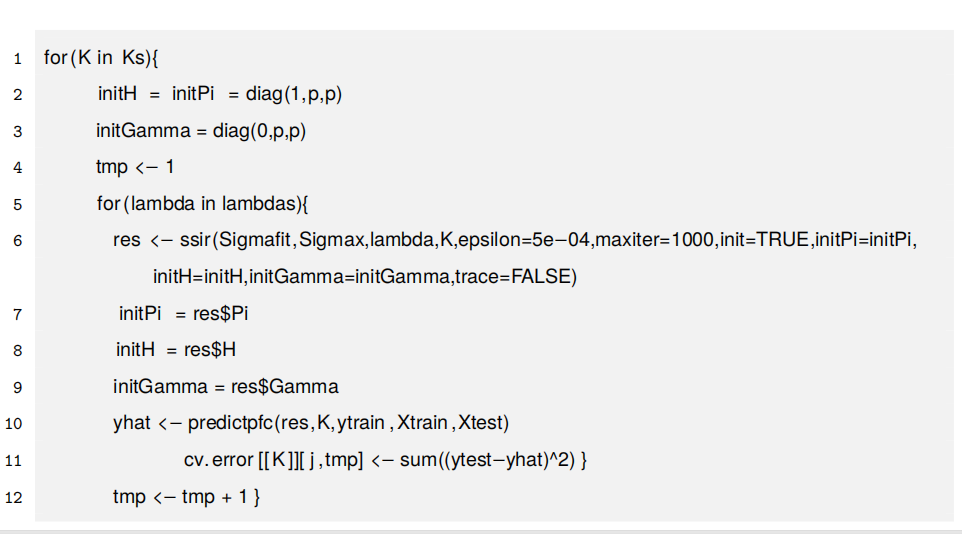
\includegraphics[scale=0.3]{code2.png}
\end{frame}
\subsection{Results}

\begin{frame}{Our reviewing results}
  \begin{itemize}
  \item \textcolor{blue}{Simulation:} observations x from $N_{d}\left(0, \Sigma_{x}\right),$ where $\left(\Sigma_{x}\right)_{i j}=0 \cdot 5^{|i-j|}$ for $1 \leqslant i, j \leqslant d, \epsilon$ from $N(0,1)$
  \item \textcolor{red}{Model 1:} $$y=\left(x_{1}+x_{2}+x_{3}\right) / 3^{1 / 2}+2 \epsilon$$
  \item \textcolor{red}{Model 2:}$$y=1+\exp \left\{\left(x_{1}+x_{2}+x_{3}\right) / 3^{1 / 2}\right\}+\epsilon$$
  \item \textcolor{red}{Model 3:}$$y=\frac{x_{1}+x_{2}+x_{3}}{0.5+\left(x_{4}+x_{5}+1 \cdot 5\right)^{2}}+0 \cdot 1 \epsilon$$

  \end{itemize}
  
\end{frame}

\begin{frame}{Our reviewing results}
    \renewcommand{\arraystretch}{1.5} 
\begin{table}[!h]

  \centering
  \fontsize{6.5}{8}\selectfont
  \caption{Demographic Prediction performance comparison by three evaluation metrics.}
  \label{tab:performance_comparison}
    \begin{tabular}{|c|c|c|c|c|c|c|}
    \hline
    \multirow{Result}&
    \multicolumn{3}{c|}{n = 100 and d = 150}&\multicolumn{3}{c|}{ n = 200 and d = 150}\cr\cline{2-7}
    &Setting 1&Setting 2&Setting 3&Setting 1&Setting 2&Setting 3\cr
    \hline
    \hline
    TPR&  94.3 & 91.2& 89.7& 96.0 & 93.7  & 94.6\cr\hline
    FPR&  4.7 &  5.1& 6.4 & 4.1 &  3.9 &4.8\cr\hline
    corr& 85.2& 81.8&  77.3& 89.5 & 88.4  &80.3\cr
    \hline
    \end{tabular}
\end{table}
\begin{itemize}
    \item \textcolor{blue}{TPR},true positive rate,means proportion of correctly identified non-zero diagonals;
    \item \textcolor{blue}{FPR},false positive rate,means proportion of zero diagonals that are incorrectly identified to be nonzeros. 
    \item\textcolor{blue}{Corr} means absolute correlation coefficient between the true sufficient predictor and its estimate. 
\end{itemize}
\end{frame}

\begin{frame}{Model 1}
    \begin{itemize}
        \item In the selection of parameter,the author didn't mention the possible parameter choosing ,so we tested a few possible sets of parameter for their iterations and getting the following picture 
    \end{itemize}
\end{frame}
\begin{frame}{Our reviewing results-Model 1}
    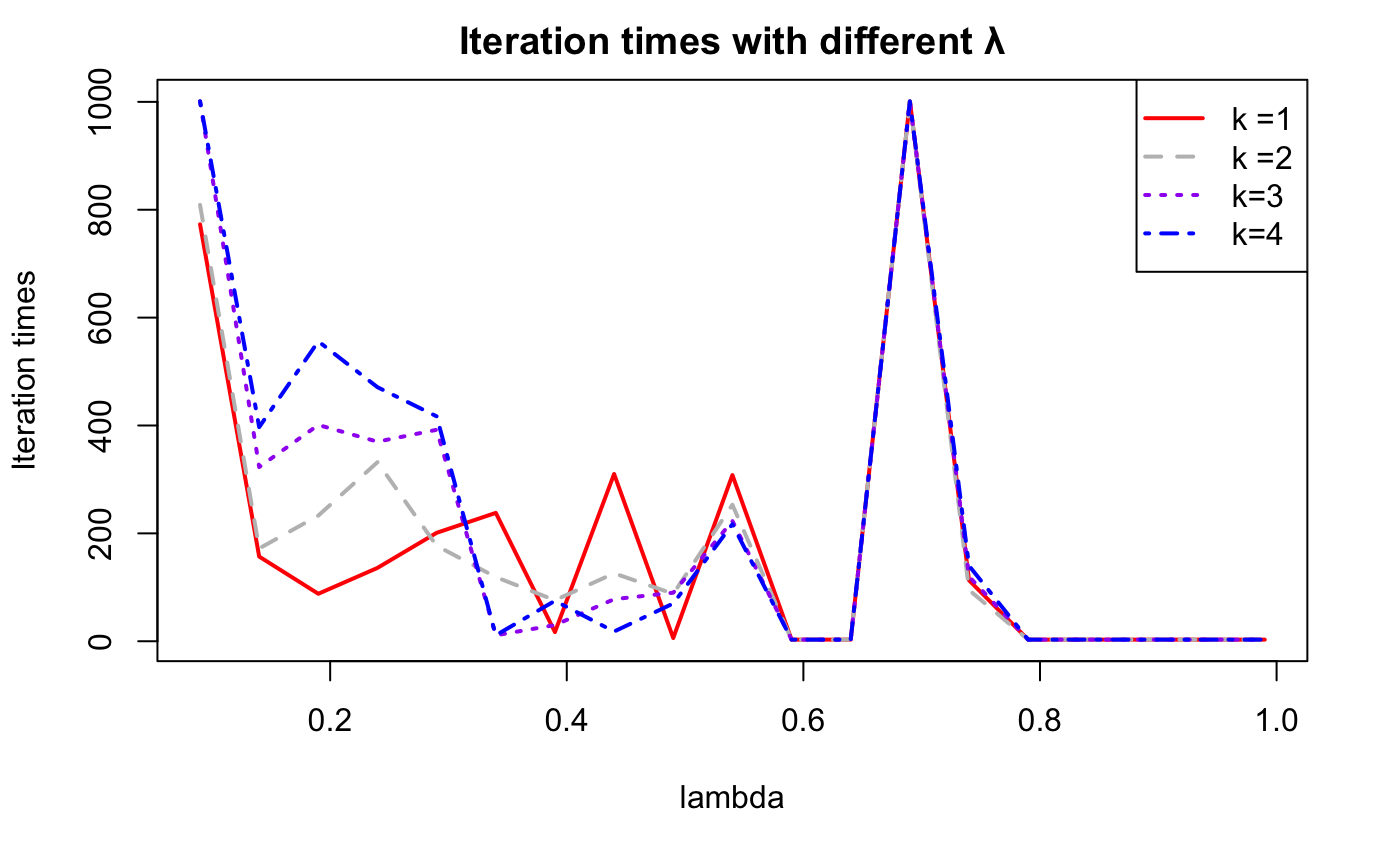
\includegraphics[scale=0.2]{plot1.png}
    \begin{itemize}
        \item we can find that choosing $\rho $ from 0.3 to 0.5 and $K\leqslant3 $ can get a good convergence.
    \end{itemize}
\end{frame}



\begin{frame}{Our reviewing results-Model 1}
    \begin{itemize}
        \item The comparison with other methods:\textcolor{blue}{Lasso,Ridge,ElasticNet regression} ;results are as follows:
    \end{itemize}
    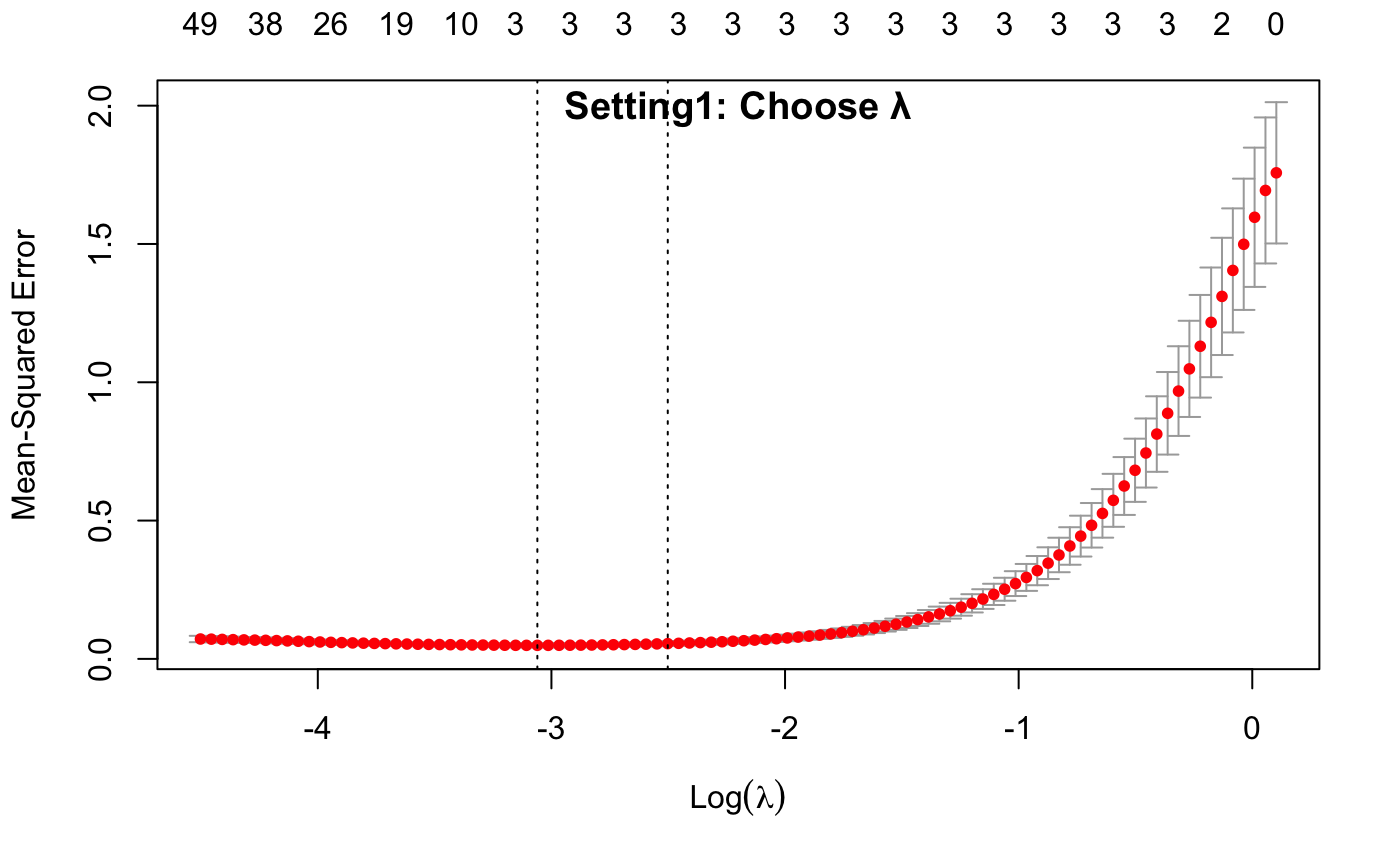
\includegraphics[scale=0.2]{1.3.png}
\end{frame}

\begin{frame}{Model 1}
    \centering 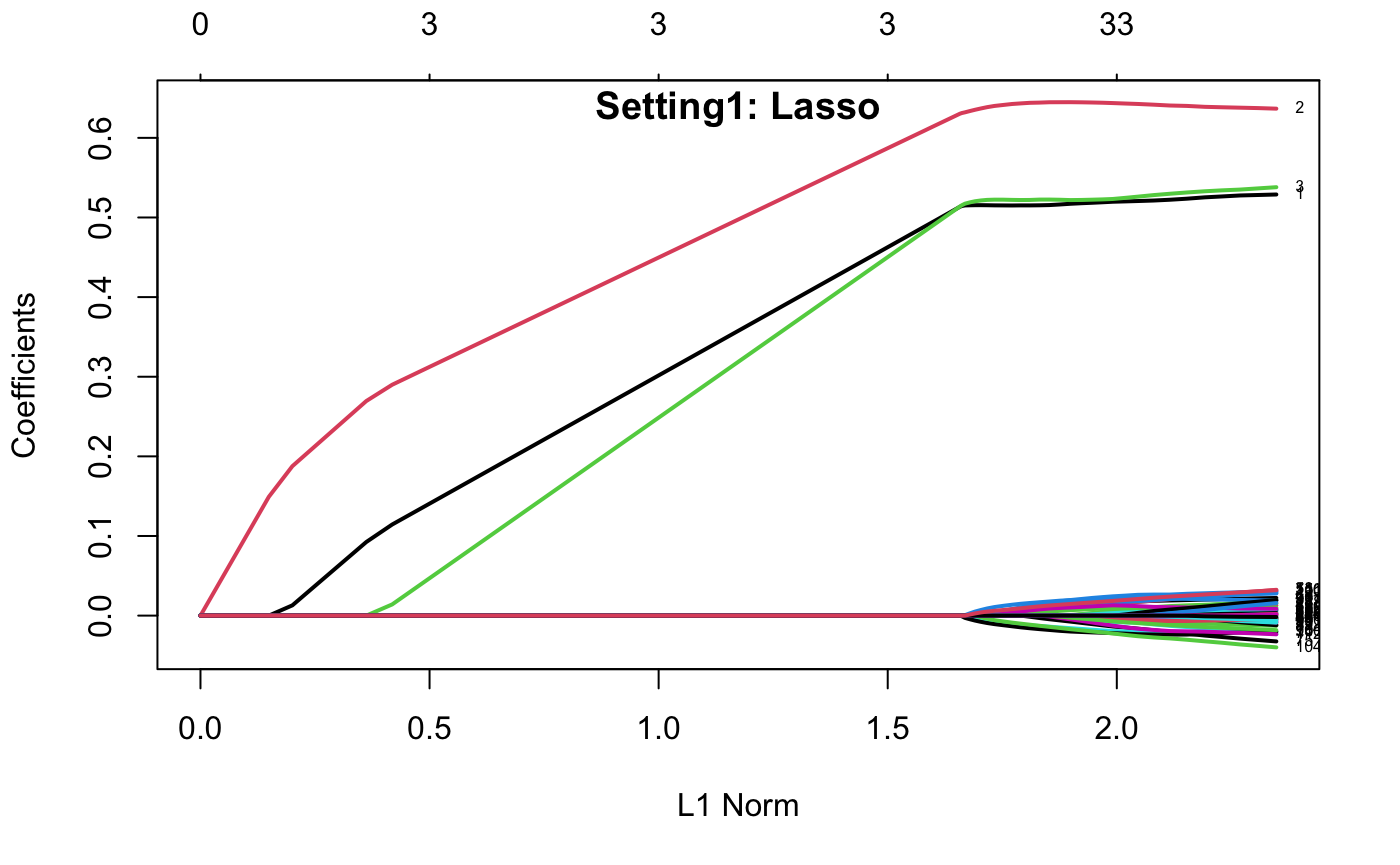
\includegraphics[scale=0.13]{1.4.png}
     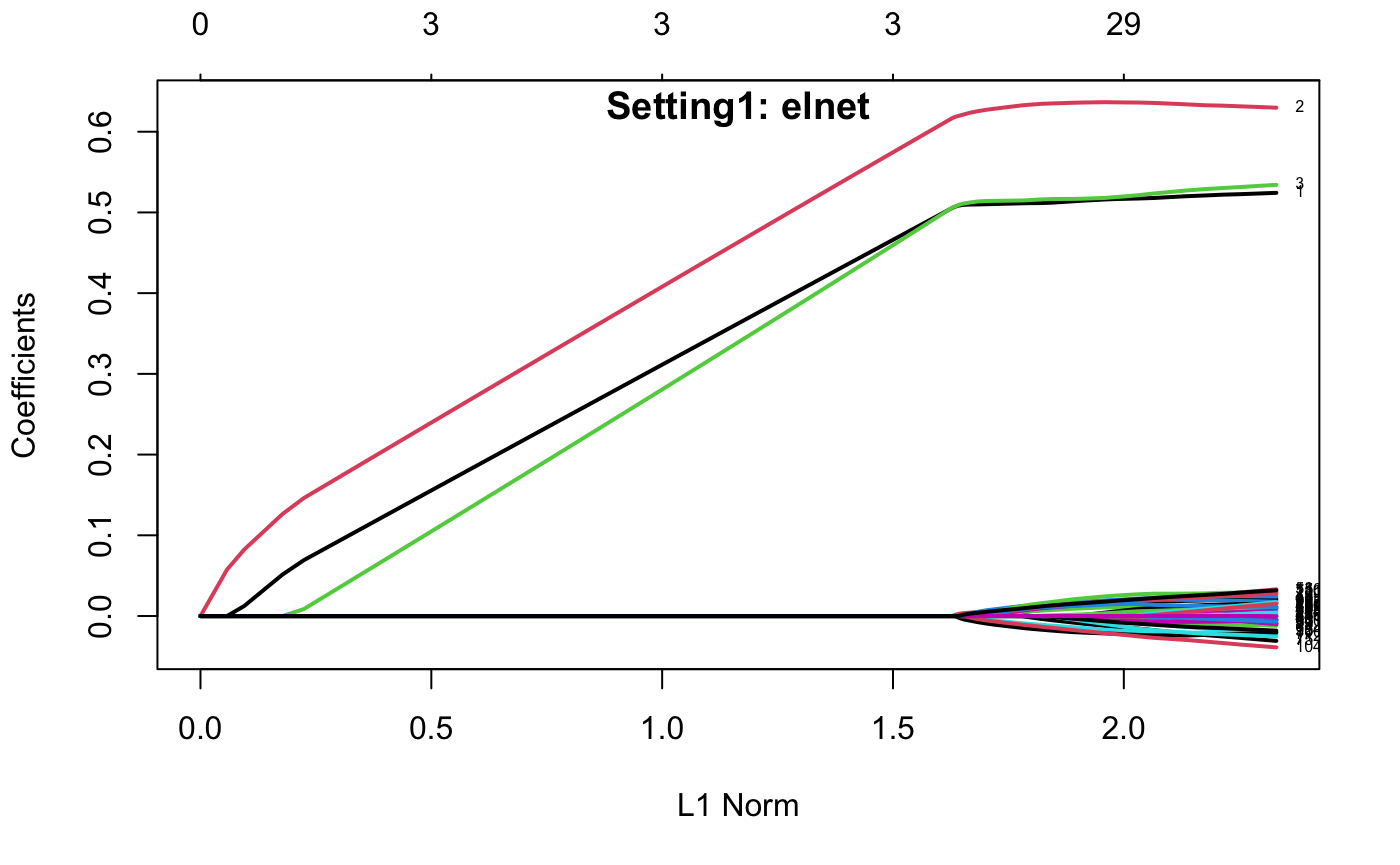
\includegraphics[scale=0.13]{1.2.png}
\end{frame}
\begin{frame}{Our reviewing results-Model 1}
    \centering 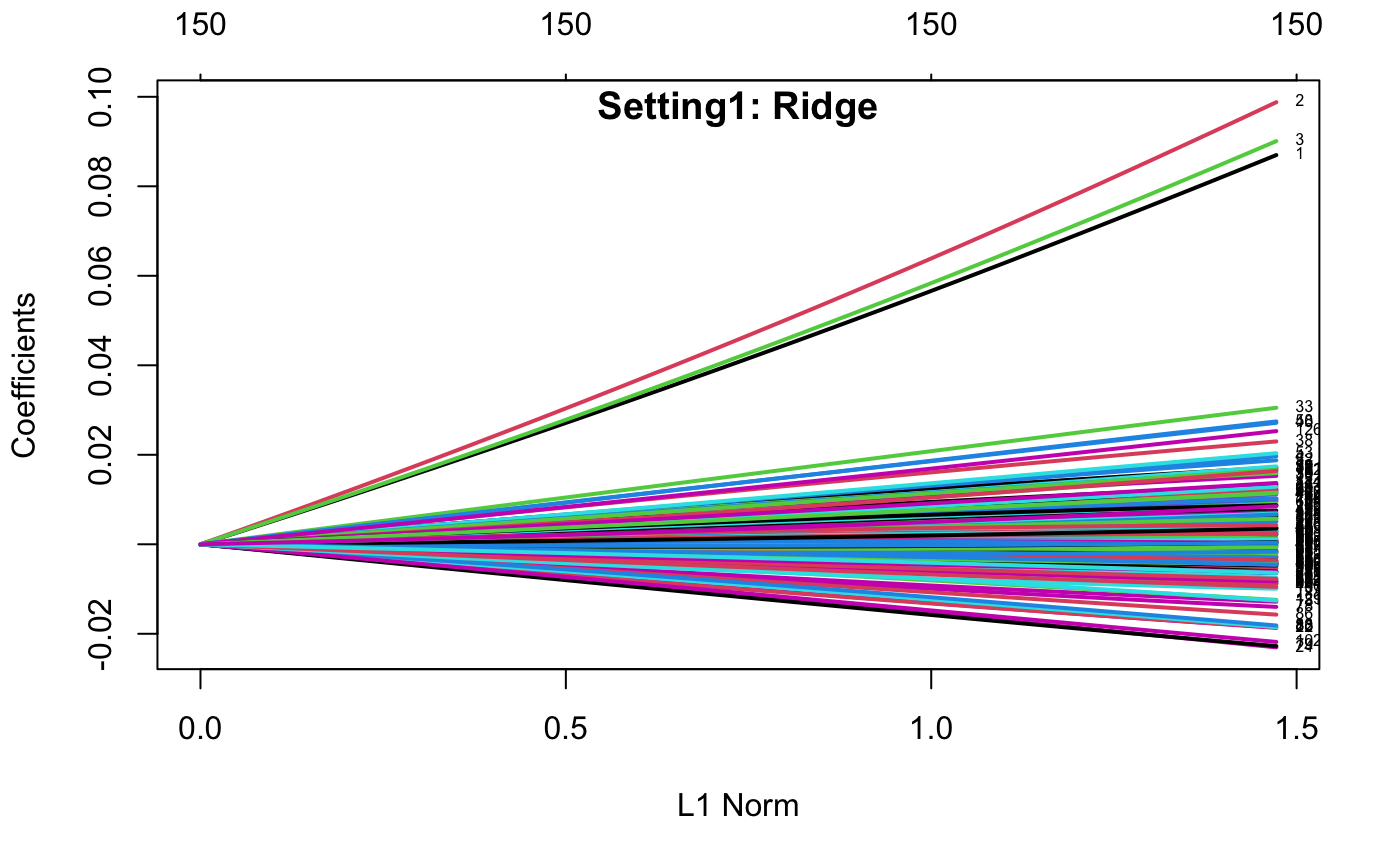
\includegraphics[scale=0.15]{1.1.png}
\end{frame}

\begin{frame}{Our reviewing results-Model 2}
    \begin{itemize}
        \item The comparison with other methods:\textcolor{blue}{Lasso,Ridge,ElasticNet regression} ;results are as follows:
    \end{itemize}
    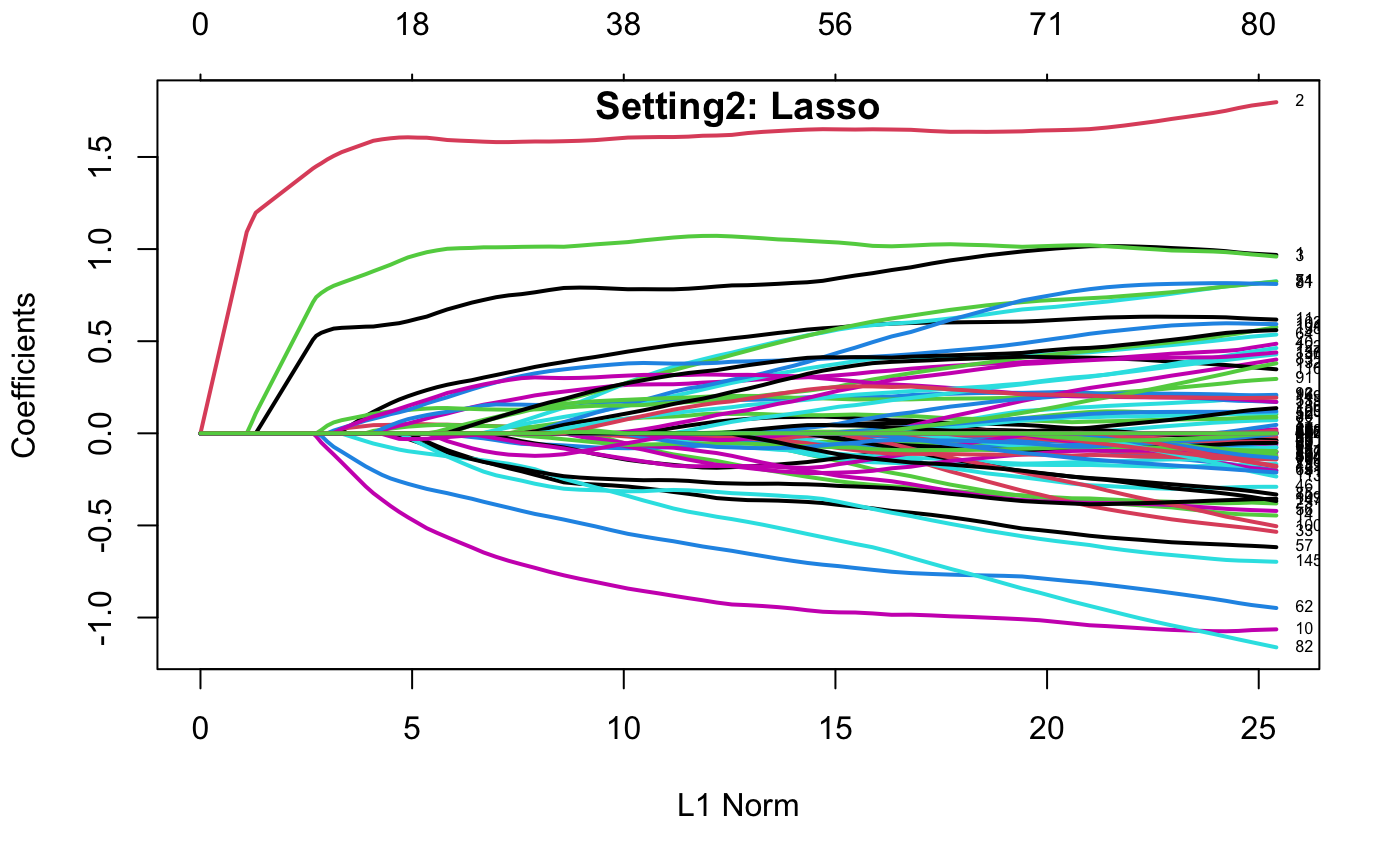
\includegraphics[scale=0.2]{2.1.png}
\end{frame}

\begin{frame}{Model 2}
    \centering 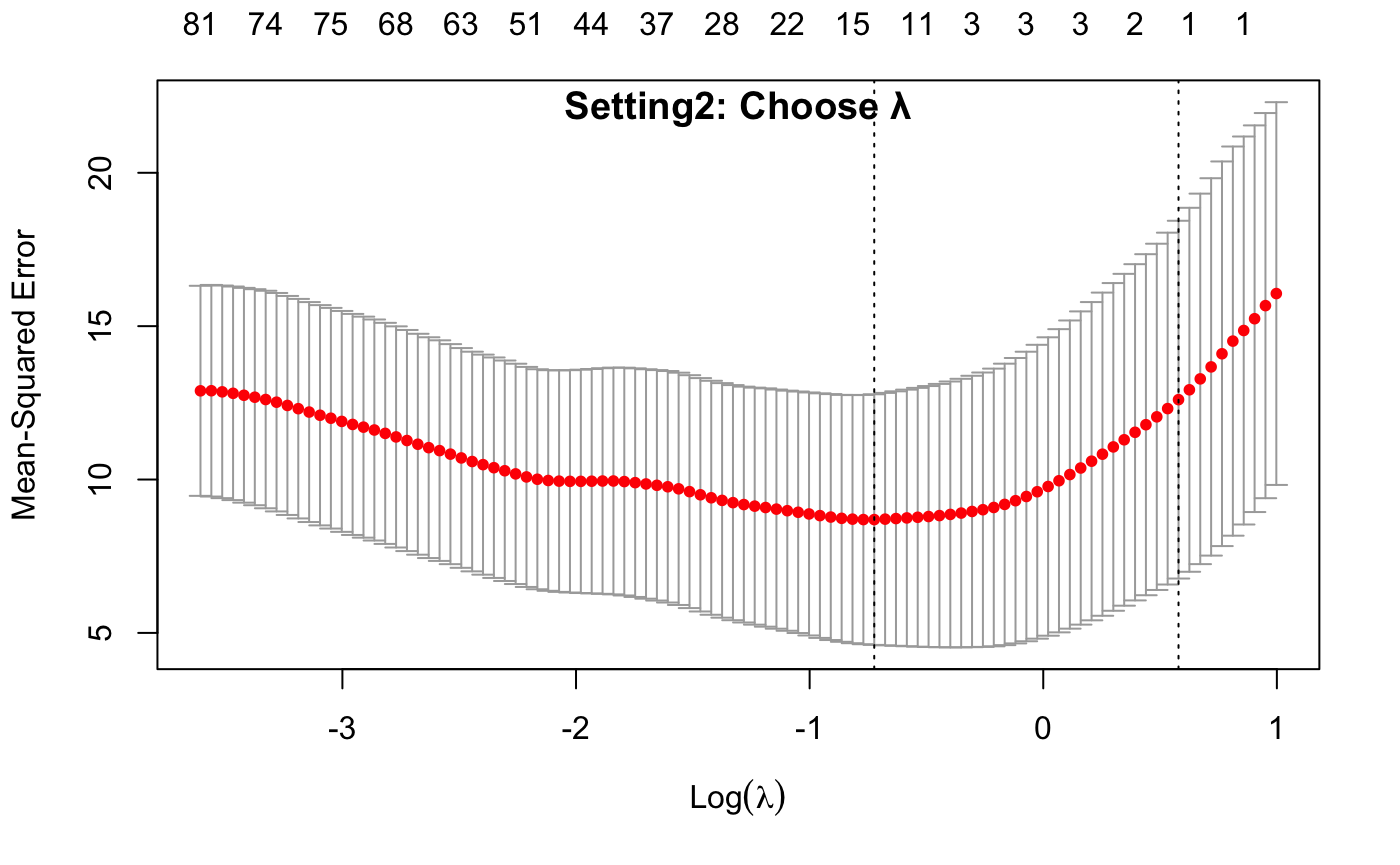
\includegraphics[scale=0.13]{2.3.png}
     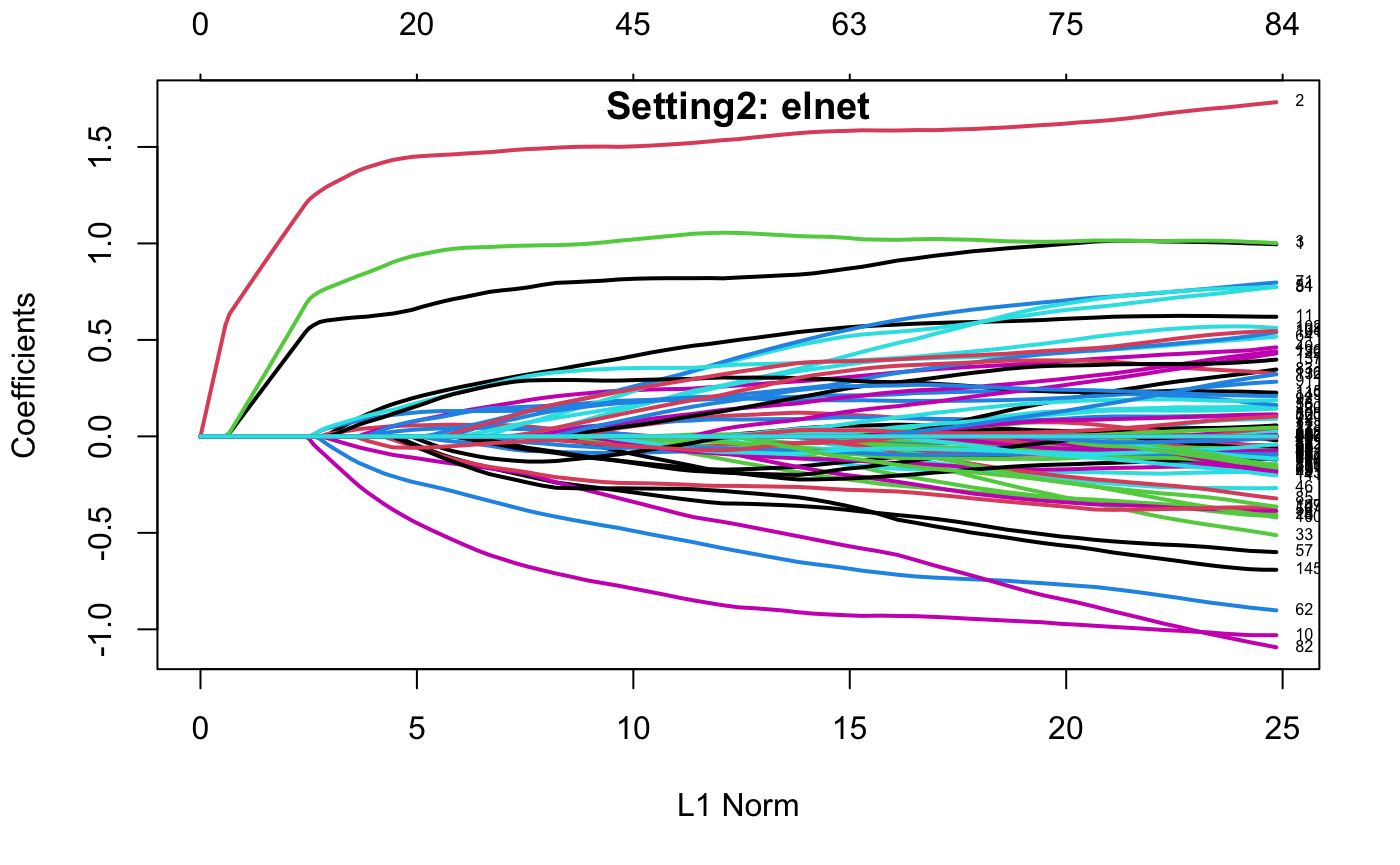
\includegraphics[scale=0.13]{2.4.png}
\end{frame}
\begin{frame}{Our reviewing results-Model 2}
    \centering 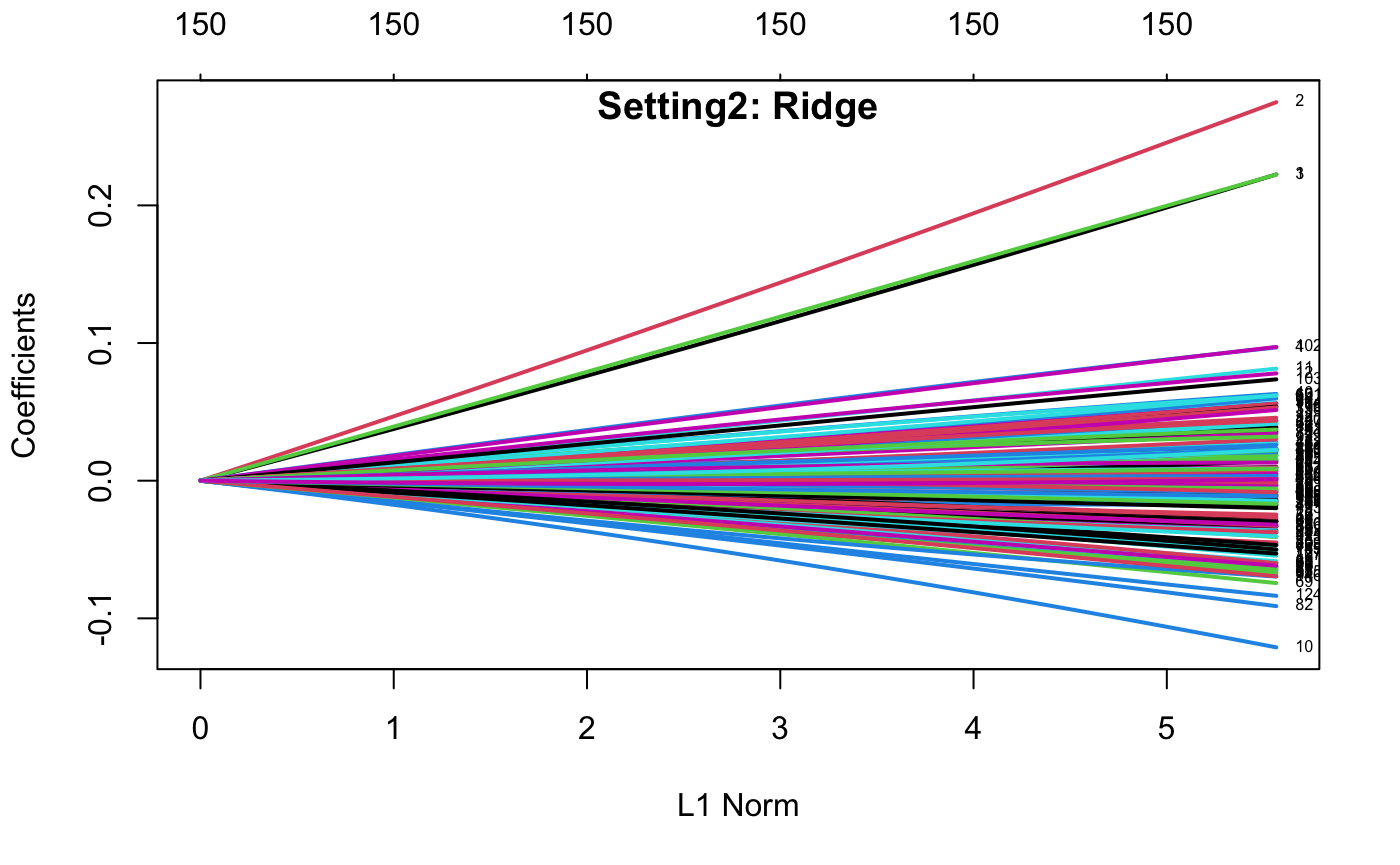
\includegraphics[scale=0.15]{2.2.png}
    \begin{itemize}
        \item We can find that in setting 2, elnet and Lasso methods are poor at choosing right subspace,while Ridge method has good result.
    \end{itemize}
\end{frame}

\begin{frame}{Our reviewing results-Model 3}
    \begin{itemize}
        \item The comparison with other methods:\textcolor{blue}{Lasso,Ridge,ElasticNet regression} ;results are as follows:
    \end{itemize}
    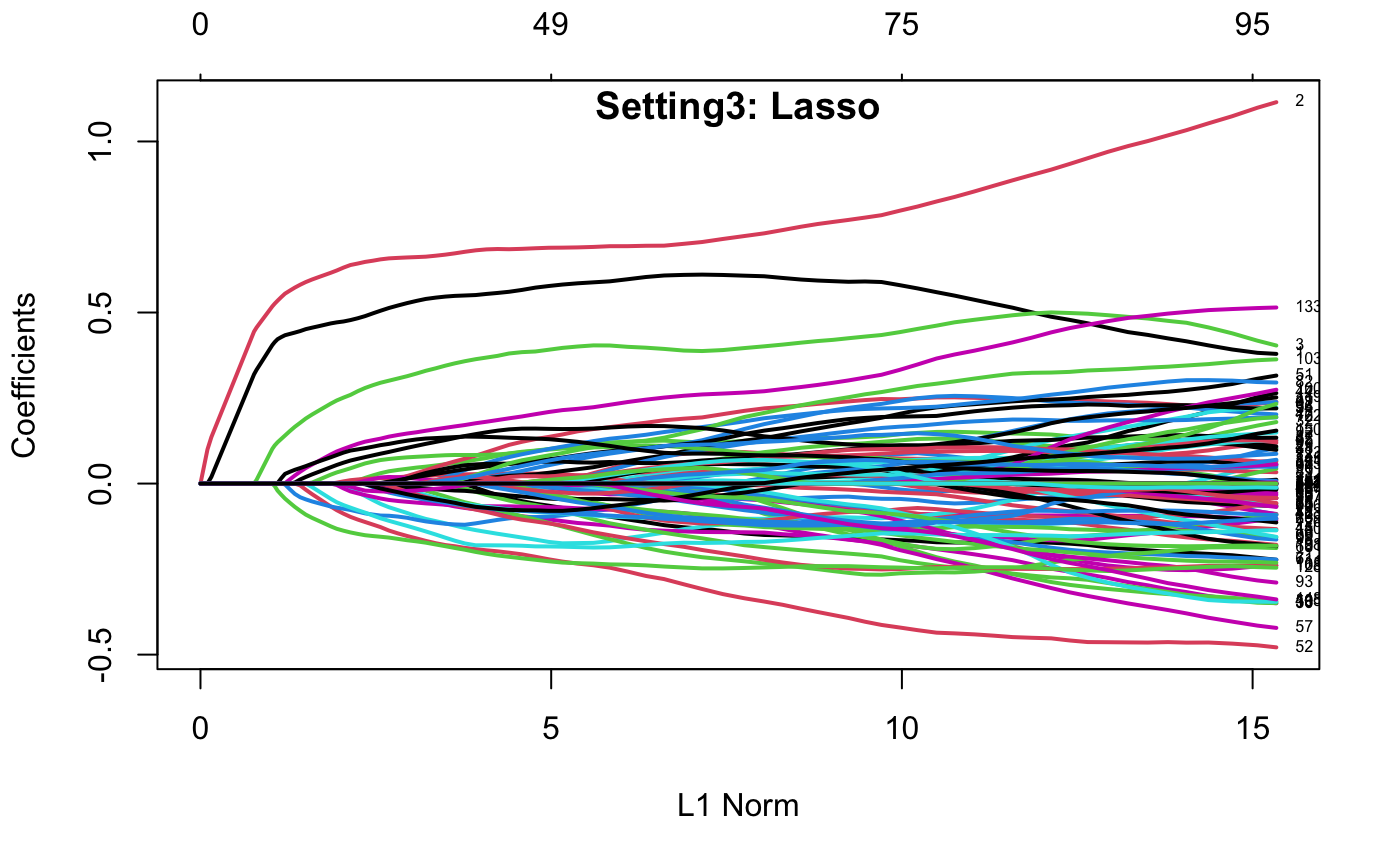
\includegraphics[scale=0.2]{3.3.png}
\end{frame}

\begin{frame}{Model 3}
    \centering 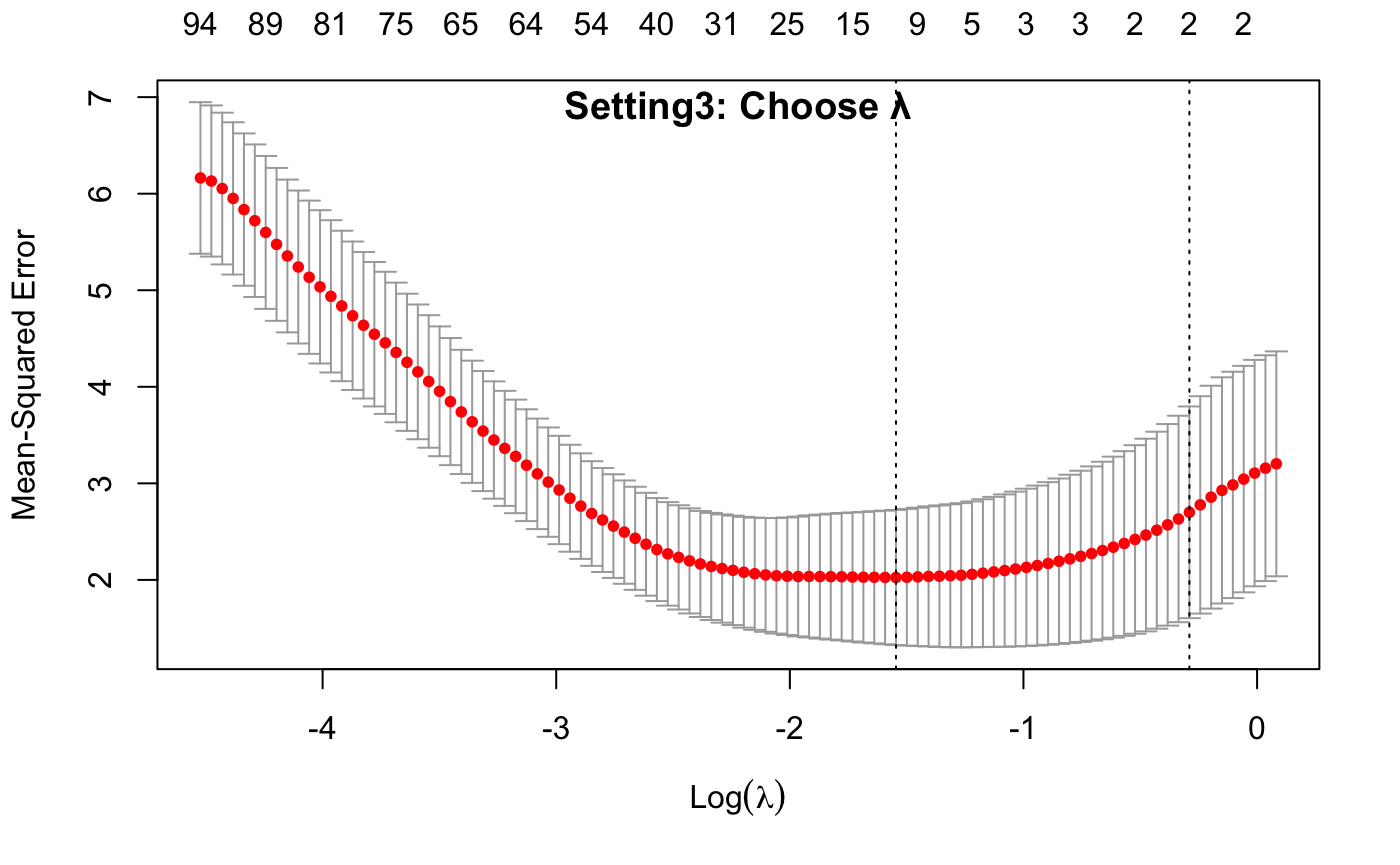
\includegraphics[scale=0.13]{3.1.png}
     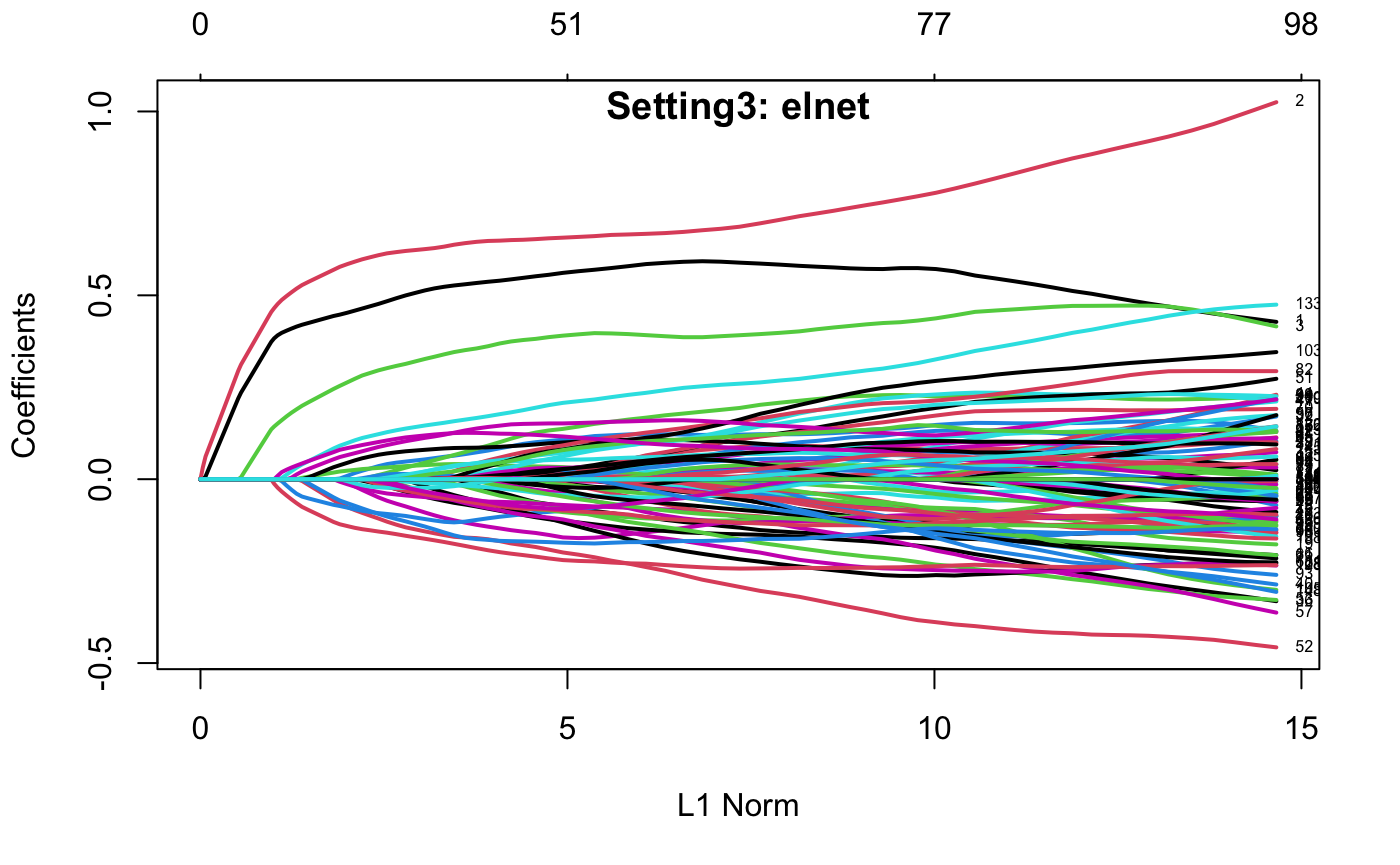
\includegraphics[scale=0.13]{3.4.png}
\end{frame}
\begin{frame}{Our reviewing results-Model 3}
    \centering 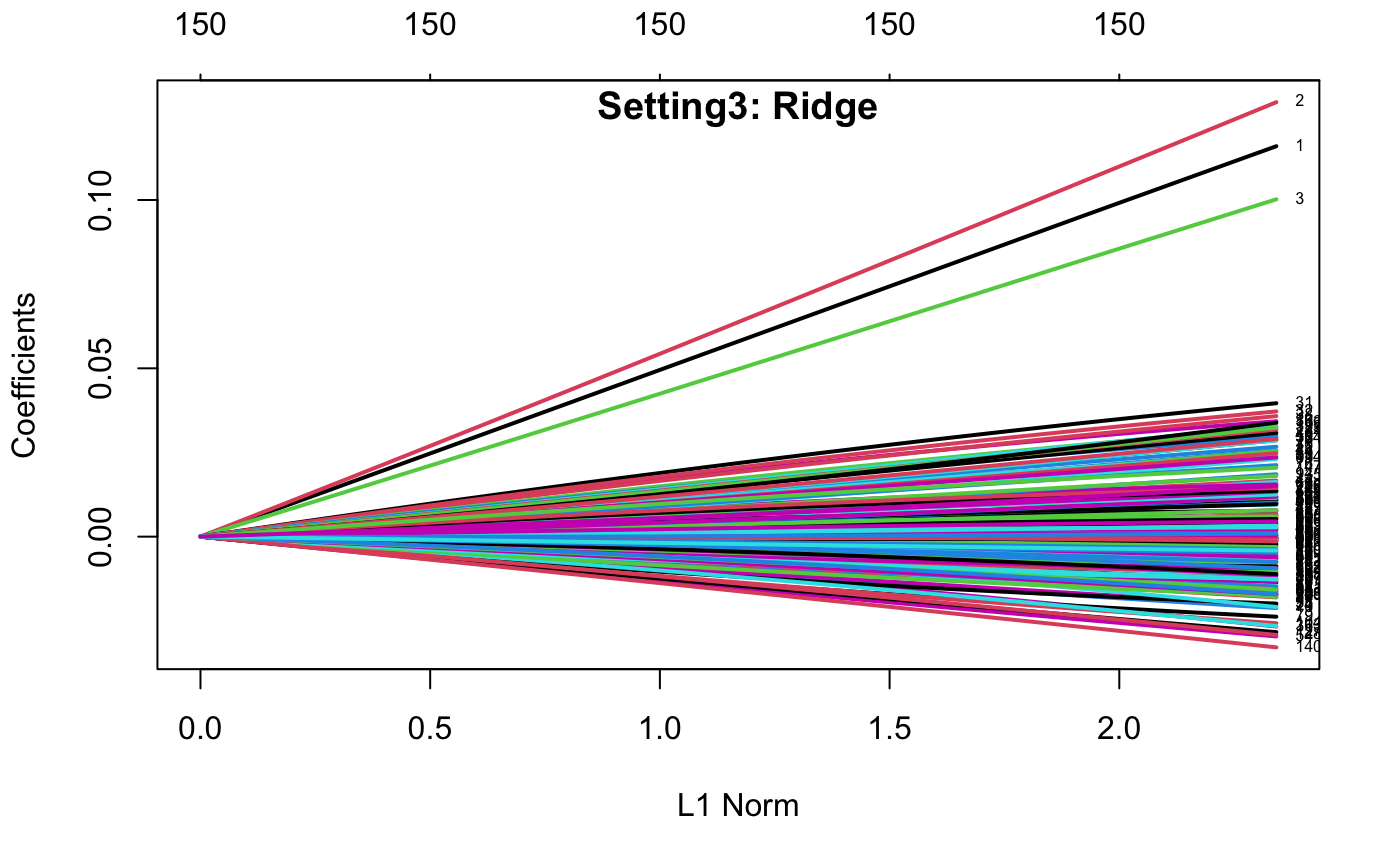
\includegraphics[scale=0.15]{3.2.png}
    \begin{itemize}
        \item We can find that in setting 3, elnet and Lasso methods are poor at choosing right subspace,while Ridge method has good result.
    \end{itemize}
\end{frame}

\begin{frame}{Subspace distance}
 \begin{itemize}
     \item To proof theorem 1 indicating that the distance between the estimated subspace and true subspace are controlled by $s(\log d / n)^{1 / 2}$
 \end{itemize}
 
 \centering 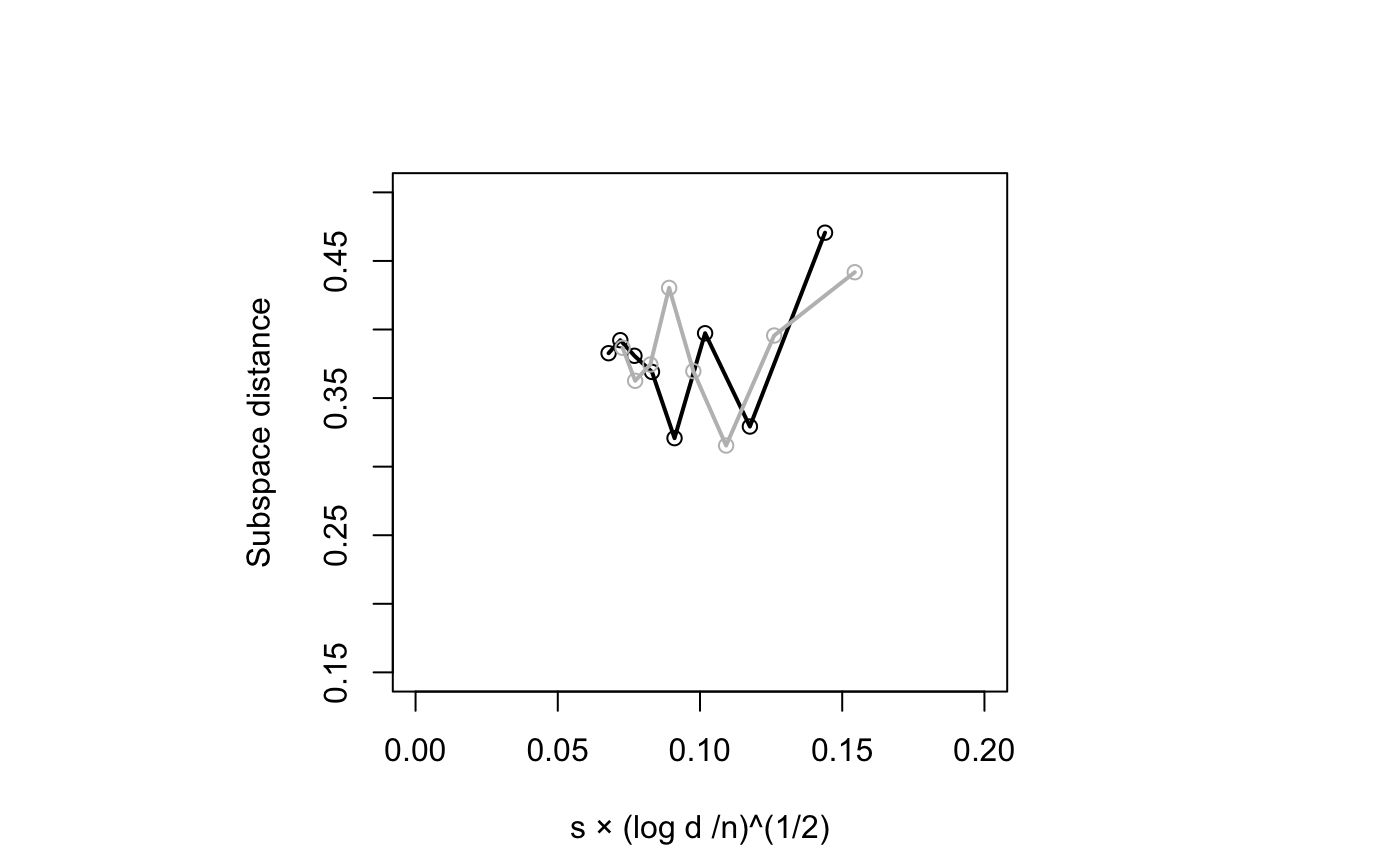
\includegraphics[scale=0.1]{41.png}
 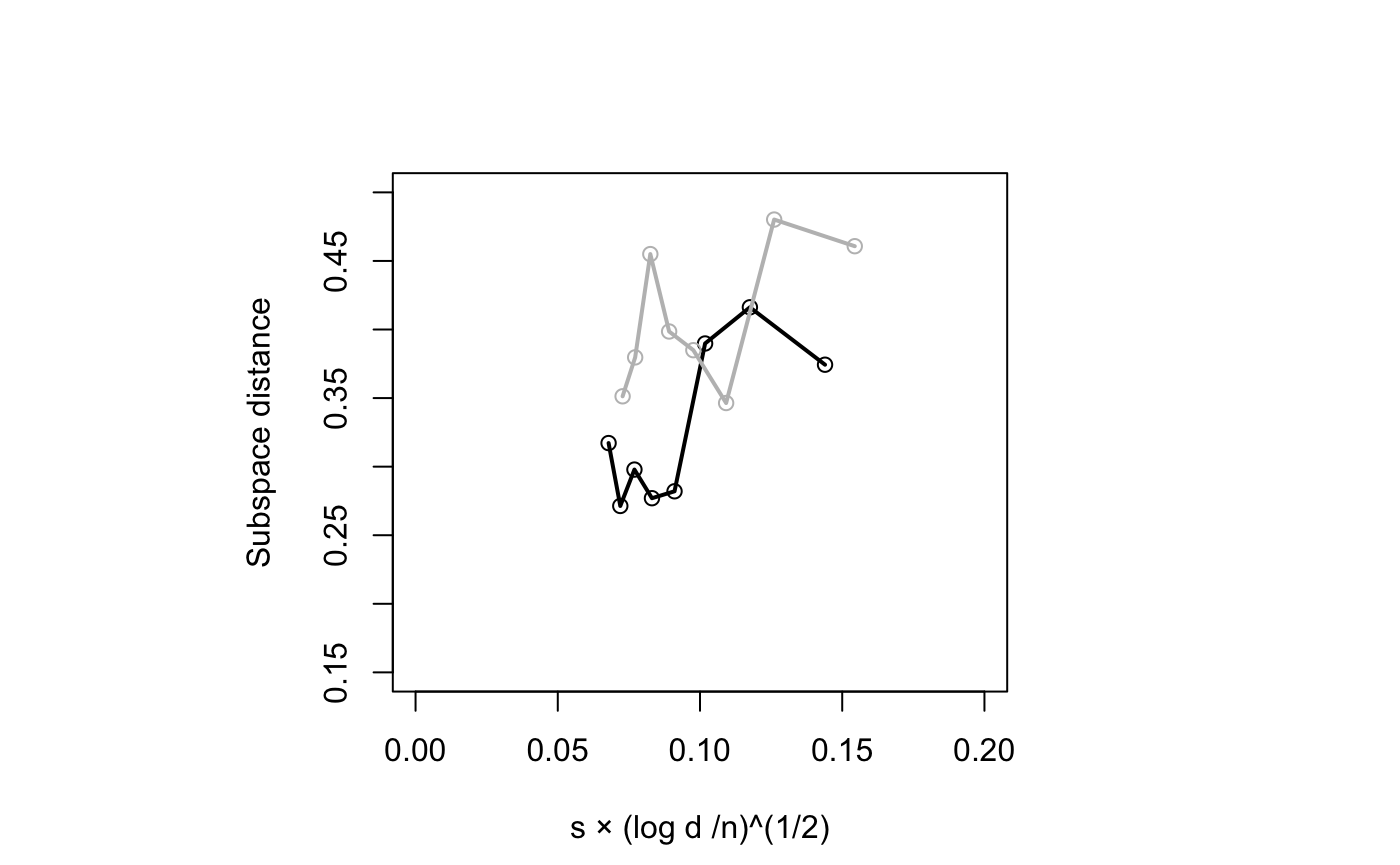
\includegraphics[scale=0.1]{42.png}
\end{frame}

\section{Conclusion}
\begin{frame}{Analysis}
    \begin{itemize}
        \item ElasticNet Regression is a method mixing $ L_1,L_2$ regularization.
$$\min _{\theta} \frac{1}{2 m}\left[\sum_{i=1}^{m}\left(\theta^{T} x^{(i)}-y^{(i)}\right)^{2}+\lambda_{1} \sum_{j=1}^{n}\|\theta\|+\lambda_{2} \sum_{j=1}^{n}\|\theta\|_{2}^{2}\right]$$
      \item We can conclude from results above that,for linear regression model, \textcolor{blue}{4 methods except Ridge} are perfect at choosing the right subspace;while for non-linear regression model,\textcolor{blue}{only the Ridge and SSIR} method can choose the right parameter.
    \end{itemize}
\end{frame}



\begin{frame}{Analysis}
    \begin{itemize}
         \item Note that our SSIR have best performance in \textcolor{blue}{both linear and non-linear} model and in both low and high dimensional setting.
        \item With comparison with other methods mentioned in paper,we can conclude,in short, that SSIR is the most \textcolor{blue}{robust} proposal across all three settings. 
    \end{itemize}
       \renewcommand{\arraystretch}{1.5} 
\begin{table}[!h]

  \centering
  \fontsize{6.5}{8}\selectfont
  \caption{Demographic Prediction performance comparison by three evaluation metrics.}
  \label{tab:performance_comparison}
    \begin{tabular}{|c|c|c|c|c|c|c|}
    \hline
    \multirow{Result}&
    \multicolumn{3}{c|}{n = 100 and d = 150}&\multicolumn{3}{c|}{ n = 200 and d = 150}\cr\cline{2-7}
    &Setting 1&Setting 2&Setting 3&Setting 1&Setting 2&Setting 3\cr
    \hline
    \hline
    TPR&  94.3 & 91.2& 89.7& 96.0 & 93.7  & 94.6\cr\hline
    FPR&  4.7 &  5.1& 6.4 & 4.1 &  3.9 &4.8\cr\hline
    corr& 85.2& 81.8&  77.3& 89.5 & 88.4  &80.3\cr
    \hline
    \end{tabular}
\end{table}
\end{frame}

\begin{frame}{Challenge and Future Work}
  \textcolor{red}{Challenge} : 
  \begin{itemize}
  \item \textcolor{blue}{Parameters choosing}:the process in choosing appropriate parameters are difficult,by several trials is not a clever way to decide possible parameters.
  \item\textcolor{blue}{Time consuming}:We find that the program takes a little long time to get results,which almost taken by Cross-validation step in selecting tuning parameters.
  \end{itemize}

  \textcolor{red}{Future work} :
  \begin{itemize}
  \item Can we get a \textcolor{blue}{rough limit} in parameter selection? So we can accelerate the program.
  \item Can SSIR be also \textcolor{blue}{robust in much higher dimensional} space? We should do more experiment to check it.
  \end{itemize}
\end{frame}

\end{document}